\section{Method}\label{sec:method}
The goal of this work is to assess the efficacy of LLMs in inverse-graphics tasks. 
We frame the problem as that of estimating a graphics program from a single image (see \cref{fig:teaser}) and fine-tune an LLM using a small, synthetic dataset.
We begin by analyzing the advantages this approach offers over traditional approaches in \cref{ssec:derendering}.
Subsequently, we delineate the details of our methodology in \cref{ssec:ig-llm}.
Finally, we elaborate on the design and motivation of the \emph{numeric head} to enable precise metric reasoning in \cref{ssec:numeric_head}.

\subsection{Traditional Neural Scene De-Rendering}\label{ssec:derendering}
Our approach builds upon the concept of neural scene de-rendering introduced by \citet{wu2017neural}.
In this framework, the goal is to develop a generalizable model capable of comprehensively understanding a scene by estimating a graphics program executable by a renderer.
NS-VQA~\citep{yi2018neural} is representative of this paradigm, where the task is addressed by decomposing the visual input using multiple modules with task-specific visual inductive biases.
The method includes several components: a region-proposal network for object detection, a segmentation network for isolating the objects from the background, an attribute network for classifying various discrete graphics attributes, and a localization network for predicting the object's spatial location.
Each network is independently trained in a supervised manner with a specific objective, and their outputs are aggregated to produce a structured representation of the scene.

\subsection{What Do LLMs Offer?}
The broad success of LLMs can be largely attributed to their exceptional ability to generalize.
Unlike models that rely on task-specific inductive biases or well-crafted training objectives, LLMs~\citep{Brown2020LanguageMA, Radford2019LanguageMA, touvron2023llama} perform proficiently across a variety of language tasks with relatively minor design differences and a simple training approach.
This success can be attributed to the scale of the models and the sets of in-the-wild data on which they are trained.

A particularly intriguing development in recent years has been the adaptation of LLMs to downstream tasks through instruction-tuning~\citep{wei_2024_instruction,Wang2022SelfInstructAL,vicuna2023}, where LLMs are fine-tuned on a small set of curated task-specific training samples (e.g., 52K instruction-following examples in Stanford Alpaca~\citep{alpaca}).
This suggests a paradigm shift from traditional approaches, where generalization is often attained by scaling the amount of task-specific training data.
LLMs are primarily trained via an unsupervised next-token-prediction objective to perform language-completion tasks, 
thereby unifying various natural language processing (NLP) tasks within a generic framework.
Our research aims to explore whether this generalized approach can be effectively extended to the task of scene de-rendering while preserving their strong generalization capabilities.

\subsection{Tuning LLMs for Inverse Graphics}\label{ssec:ig-llm}
While LLMs are traditionally trained to complete language-token sequences, VQA works~\citep{Alayrac2022FlamingoAV, Li2022BLIPBL, liu2023llava} have demonstrated that large pretrained vision transformers~\citep{ Dosovitskiy2020AnII, radford2021learning} can be efficiently adapted as visual tokenizers.
Such works unify image and language understanding, interleaving visual embeddings with language tokens for the LLM.
In line with this approach, we adopt a similar strategy, constructing an LLM capable of ``seeing'' the input image and returning a structured code representation of the input scene.

In the subsequent paragraphs, we detail the base architecture, elucidate the process of vision--language alignment, and introduce our methodology for preparing synthetic data for visual instruction finetuning.
A high-level overview of our pipeline can be seen in \cref{fig:teaser}.

\noindent\textbf{Architecture.}
Our model is based on an instruction-tuned variant~\citep{peng2023instruction} of LLaMA-1 7B~\citep{touvron2023llama} in conjunction with a frozen CLIP~\citep{radford2021learning} vision encoder, serving as the visual tokenizer.
We apply a learnable linear projection to link the vision embeddings with the word-embedding space of the LLM.

\noindent\textbf{Vision--Language Alignment.}
The linear vision-encoder projection is initially trained using the feature-alignment pre-training method from LLaVA~\citep{liu2023llava}.
This training uses instruction sequences constructed from image--caption pairs sourced from the Conceptual Captions dataset (CC3M)~\hbox{\citep{sharma2018conceptual}}.
The LLM receives the projected image embedding, followed by a randomly sampled directive tasking the model to describe the image and its corresponding caption.
Throughout this stage, all model parameters remain fixed except for the learnable vision projector.
To ensure the generality of our model, we refrain from additional instruction tuning following this initial feature alignment.

\noindent\textbf{Training-Data Generation.}
CLEVR~\citep{johnson2017clevr} is a procedurally generated dataset of simple 3D objects on a plane.
The primitives are assigned randomly sampled attributes such as shape (sphere, cube, and cylinder), size, color, material, and spatial pose.
Shape, size, color, and material are discrete attributes, while pose is a continuous parameter specifying the object's location and orientation.
The images from the sampled scenes are rendered using the \citet{blender} modeling software from its Python scripting API.
Our domain-specific language consists of \texttt{add} functions, facilitating the insertion of objects with specified attributes into the scene using Blender.
See \cref{fig:teaser} for an example of the representation of a single object.

To train our model, we generate pairs of rendered images and their corresponding code, prompting the model with the rendered image followed by the question, ``What Python Blender code could be used to produce the scene?''.
The model is then trained with a standard next-token prediction objective~\citep{bengio_plm}, aiming to maximize the conditional probability of the next token given the previous ones:
\begin{equation}\label{eq:next-token}
p(x) = \prod_{i=1}^n p\left(s_i|s_1,\ldots s_{i-1}\right) ,
\end{equation}
where $s_i$ represents the $i$th token.
Numbers are rendered with three decimal places in the text-based (tokenized) training data.
We order the \texttt{add} statements front-to-back in the objective token sequence and shuffle the order of the object attributes.
See \cref{fig:code_clevr,fig:code_2d,fig:code_so3,fig:code_single_6dof,fig:code_scene_6dof} for complete examples of each task.

\noindent\textbf{Differences From Traditional Approaches.}
The framework presented in this study marks a departure from conventional approaches.
Notably, the visual-encoding process does not include graphics-specific inductive biases in its design.
It undergoes no training for intermediate vision tasks, such as object detection, segmentation, or attribute regression.
The model operates solely on rendered images without access to 3D assets.
Moreover, the supervised fine-tuning process employs a training objective not directly related to the physical representation of the scene.

We show in \cref{sec:evaluations} that these departures do not impede performance or generalization capabilities compared with traditional approaches; in fact, they enhance them.
Our experiments demonstrate a compositional-generalization ability without the need for tailor-made designs, surpassing the conventional approach by approximately 60\% in OOD shape-recognition accuracy.

\subsection{Precise Numeric Reasoning in LLMs}\label{ssec:numeric_head}
\begin{figure}[t]
\centering
\begin{subfigure}{0.5\linewidth}
\centering
\raisebox{1.05cm}{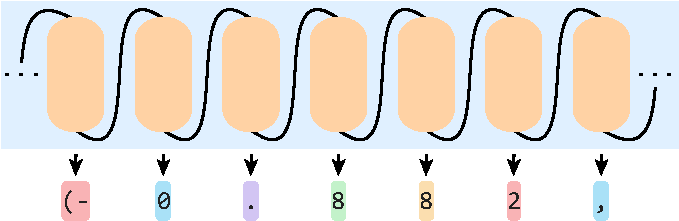
\includegraphics[width=\linewidth]{figures/diagram/not_numeric_head.pdf}}
\caption{Discretized numerics}
\label{fig:not_numeric_head}
\end{subfigure}
\hspace{1cm}
\begin{subfigure}{0.2350\linewidth}
\centering
\vspace{0.1cm}
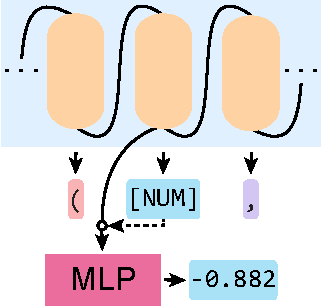
\includegraphics[width=\linewidth]{figures/diagram/numeric_head_diagram.pdf}
\caption{Continuous numerics}
\label{fig:numeric_head}
\end{subfigure}
\caption{\textbf{Numeric Head.} (\cref{ssec:numeric_head})
Rather than producing digits as discrete tokens (a), we train our model to generate a [NUM] token when a number should be produced.
The [NUM] token is used as a mask to signal the embedding should instead be passed through the numeric head, preserving the gradient (b).
}
\end{figure}
Graphics programming requires the precise estimation of continuous quantities such as location and orientation, along with a comprehension of Euclidean space.
This requirement extends beyond the coarse, semantic-level spatial reasoning (e.g.~``left,'' ``in front of'') for which LLMs are typically employed, in tasks such as VQA~\citep{Antol_2015_ICCV}.
Estimating continuous values through character-based outputs essentially transforms the task into a discrete, combinatorial challenge.
In this loss space, prediction errors do not reflect real metric distances -- a ground truth value of `4' is considered as close to a prediction of `3' as it is to `8,' highlighting the inherent limitations of this approach for tasks demanding high numerical precision.

To address this challenge, we introduce a \emph{numeric head} tailored to enable continuous parameter estimation.
A visual representation of the numeric-head integration is depicted in \cref{fig:numeric_head}, contrasting with the discrete text-based alternative.
The module is implemented as a four-layer MLP that processes the final hidden-layer output of the LLM and transforms it into a scalar value.
To allow the LLM to discern between generating numerical values or textual information, we designate a special token in the vocabulary -- [NUM] -- which serves as a mask to indicate whether a number should be produced.
During training, we apply an MSE loss on each number in addition to the next-token prediction loss (\cref{eq:next-token}) used on the [NUM] token itself.

We systematically investigate the behavior of character-based and numeric IG-LLM variants for precise spatial reasoning in \cref{ssec:parameter_space_generalization}.
Our empirical findings support our intuition regarding the limitations of the character-based output and demonstrate that the numeric head enables strong generalization when the testing samples are OOD in parameter space.
These differences are highlighted throughout our evaluation.